\section{Putting it all together: Experience of PanDA on TITAN} % (fold)
\label{sec:panda_titan}

\subsection{PanDA Metadata Performance Impact at OLCF}


The ATLAS framework has a configuration and initialization stage, which is
called Athena. At this stage, the running job is assembled  on the fly from a
large number of shared libraries.  Also, at this stage, every algorithm and
service is being configured, at run time, by a corresponding set of Python
scripts, which results in a large number of read I/O accesses to small python
scripts, with many includes and imports Python calls.

When ATLAS was originally deployed at the OLCF, all shared libraries were
placed at the Spider 2 Lustre file system. However, it was quickly discovered
that the I/O pattern at the Athena stage was detrimental to the overall Spider
2 performance. Since Spider 2 is a center-wide file system and shared by all
OLCF resources and users, this resulted in lower overall interactive and
metadata performance at OLCF. As can be seen in Listing~\ref{mdstrace} the
metadata I/O activity for ATLAS exhibits a spike corresponding to the beginning
of the runs (i.e., the Athena stage) before tapering off.

\begin{lstlisting}[language=bash,frame=single,basicstyle=\ttfamily\tiny,caption=ATLAS metadata trace,label=mdstrace] 
XK7 Application 9205593
      39012 RPCs from 300 of 300 nodes
        ~69291.96 per sec
          37851 LDLM_ENQUEUE RPCs    ~67229.83 per sec
                pmin 13us pavg 42us pmax 4983us
          611 LDLM_CANCEL RPCs    ~1085.24 per sec
                pmin 10us pavg 16us pmax 32us
          277 MDS_CLOSE RPCs    ~492.00 per sec
                pmin 15us pavg 20us pmax 38us
          154 MDS_READPAGE RPCs    ~273.53 per sec
                pmin 170us pavg 292us pmax 671us
          86 MDS_GETXATTR RPCs    ~152.75 per sec
                pmin 15us pavg 21us pmax 65us
          30 MDS_GETATTR RPCs    ~53.29 per sec
                pmin 16us pavg 20us pmax 27us
          3 MDS_REINT RPCs    ~5.33 per sec
                pmin 103us pavg 136us pmax 196us
          Overall times
                pmin 10us pavg 42us pmax 4983us

XK7 Application 9205355
      8698 RPCs from 62 of 62 nodes
        ~15449.13 per sec
          8445 LDLM_ENQUEUE RPCs    ~14999.76 per sec
                pmin 16us pavg 41us pmax 780us
          92 MDS_CLOSE RPCs    ~163.41 per sec
                pmin 15us pavg 23us pmax 52us
          55 MDS_READPAGE RPCs    ~97.69 per sec
                pmin 189us pavg 291us pmax 534us
          52 LDLM_CANCEL RPCs    ~92.36 per sec
                pmin 12us pavg 16us pmax 25us
          41 MDS_GETXATTR RPCs    ~72.82 per sec
                pmin 16us pavg 20us pmax 27us
          13 MDS_GETATTR RPCs    ~23.09 per sec
                pmin 16us pavg 21us pmax 38us
          Overall times
                pmin 12us pavg 42us pmax 780us

\end{lstlisting}

As this problem was identified, the OLCF staff has enabled read-only access to
certain NFS-exported directories from Titan compute nodes. This in turn allowed
the OLCF staff to install a software package from a Titan login node and have
it available read-only on a Titan compute node.  

After moving the ATLAS release on Lustre to the NFS-exported read-only
directories, the metadata contention problem has resolved and a two orders of
magnitude metadata performance improvement (i.e., ~6,300 seconds on Lustre vs.
~1,500 seconds on NFS) has been observed for ATLAS.  Also, for both cases the
input file is placed on memory disk on a Titan compute nodes and for Lustre the
validation step took on average 1,320 seconds, while it was 40 seconds on NFS,
showing a three orders of magnitude performance improvement. 

Figure~\ref{fig:atlas-perf-improvement} shows the overall ATLAS performance
improvement on Titan. The circled region illustrates the switch from Lustre to
NFS-exported directory for hosting the ATLAS release.

\begin{figure}[!htb]
    \centering
    \begin{tabular}{cc}
        {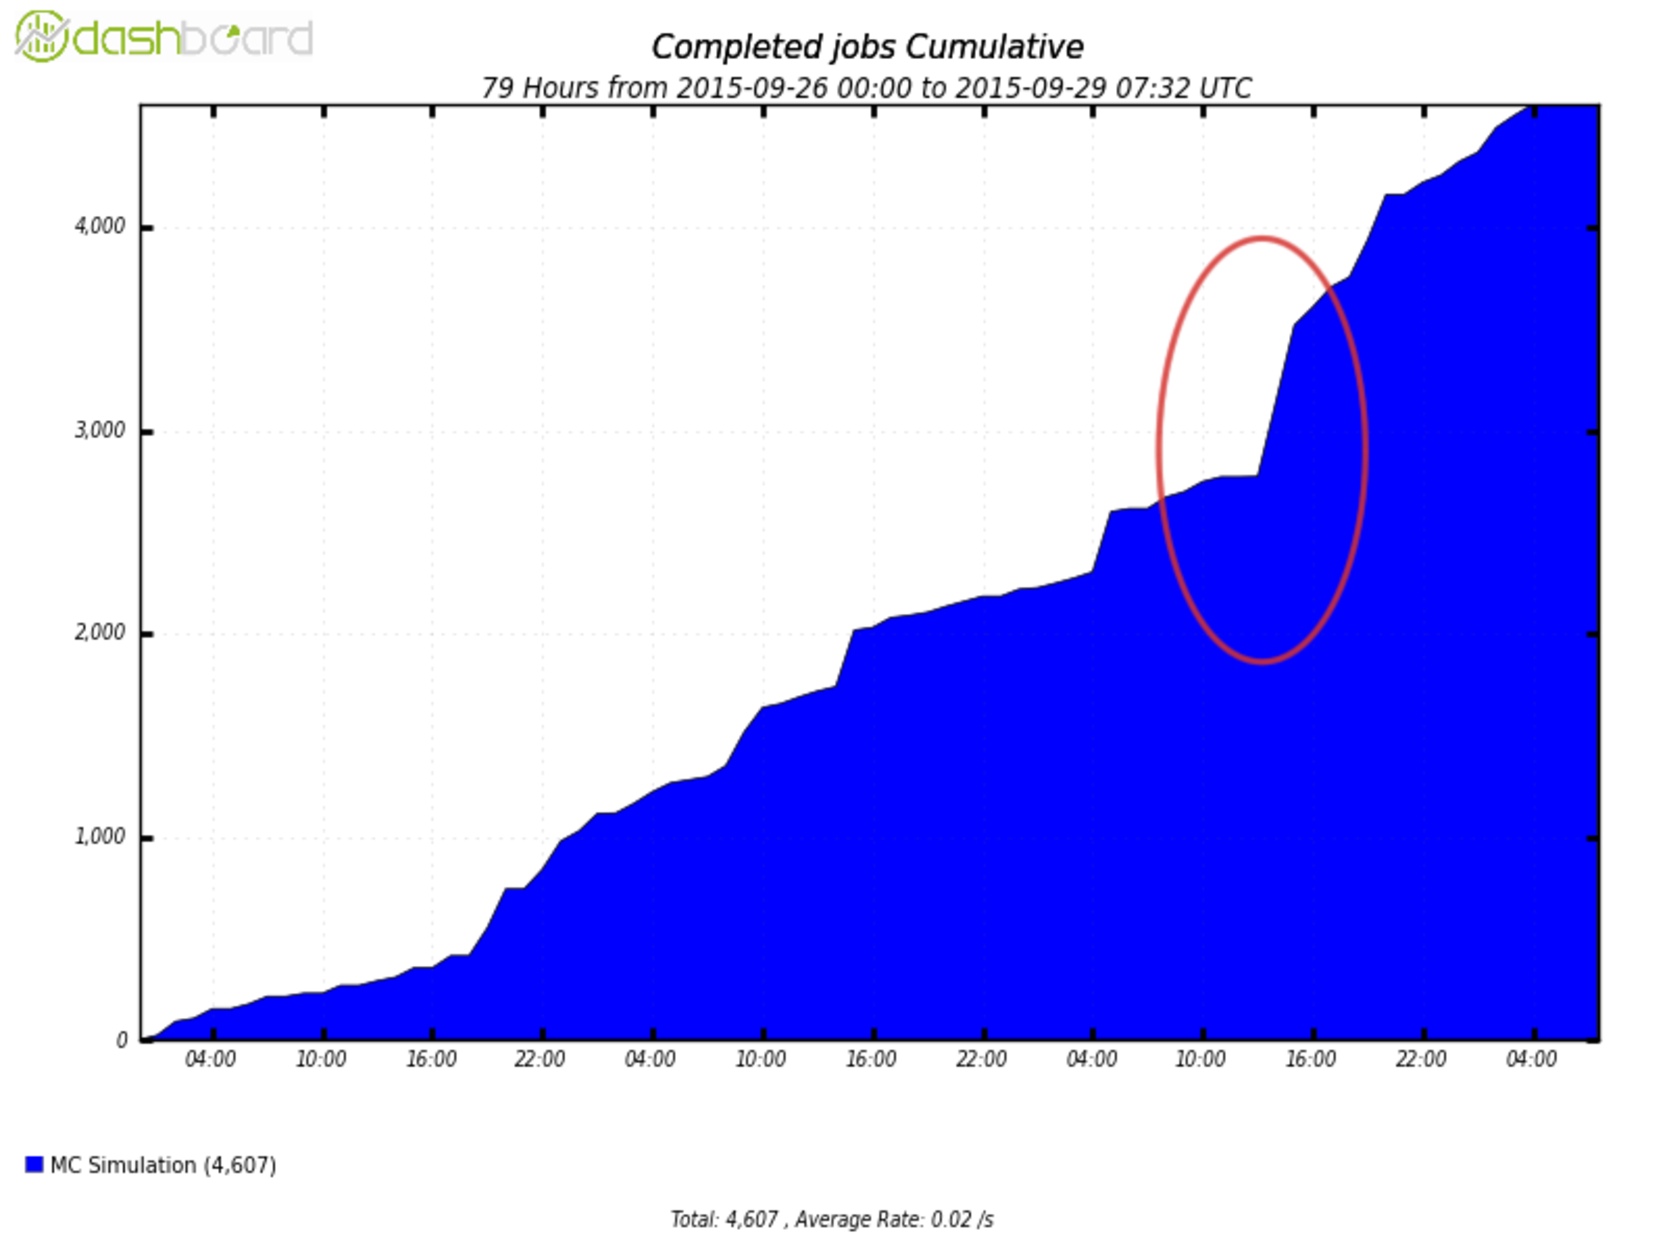
\includegraphics[width=0.48\textwidth]{figures/panda-completed-jobs-sw-move.pdf}}\\
    \end{tabular}
    \caption{ATLAS performance improvement on Titan. The circled region shows the switch from Lustre to NFS-exported directory for hosting the ATLAS release.}
    \label{fig:atlas-perf-improvement}
\end{figure}



\subsection{PanDA File I/O Performance Impact at OLCF}

File I/O performance and impact


\begin{figure}[!htb]
    \centering
    \begin{tabular}{cc}
        {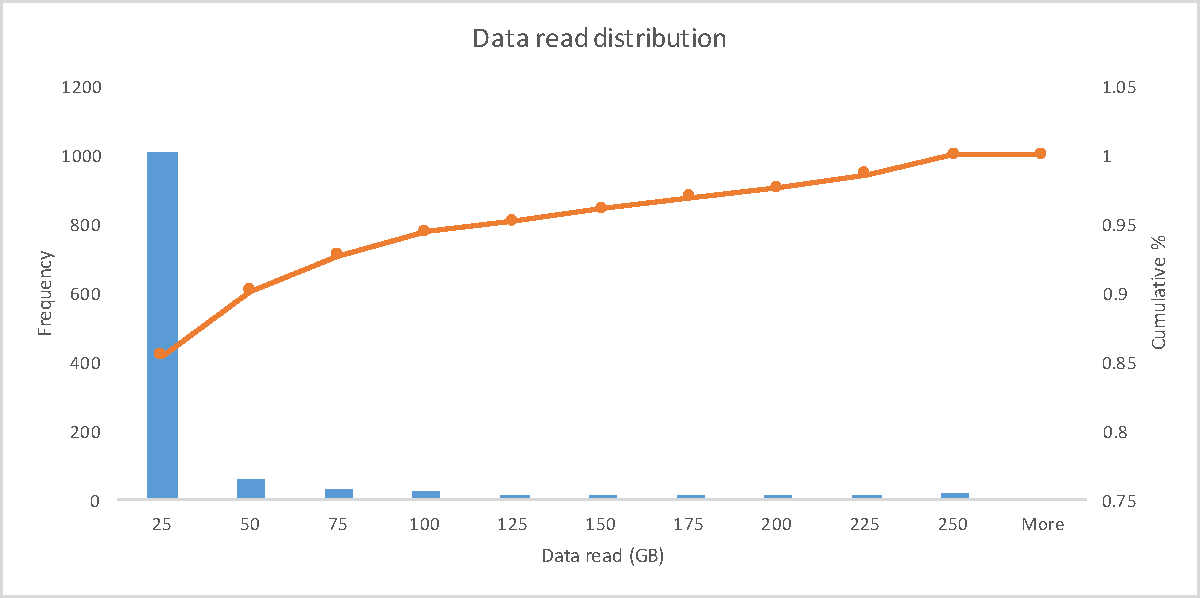
\includegraphics[width=0.48\textwidth]{figures/panda_data_read_hist.pdf}}\\
    \end{tabular}
    \caption{ATLAS file read I/O histogram on Titan for week of 10/25/16.}
    \label{fig:atlas-titan-io-read}
\end{figure}



\begin{figure}[!htb]
    \centering
    \begin{tabular}{cc}
        {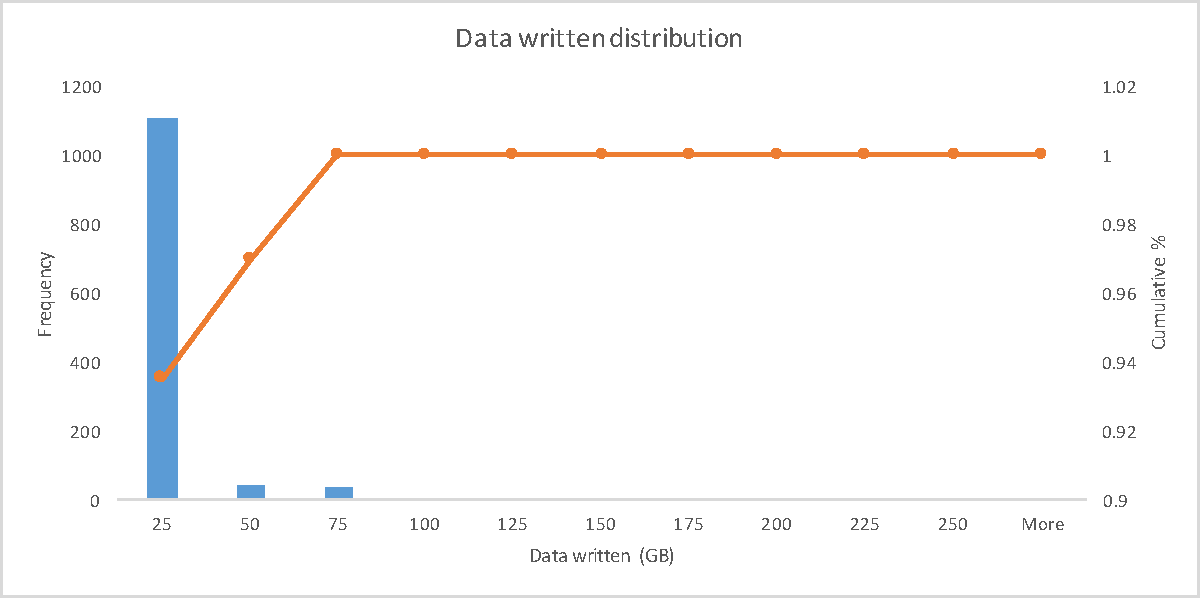
\includegraphics[width=0.48\textwidth]{figures/panda_data_written_hist.pdf}}\\
    \end{tabular}
    \caption{ATLAS file write I/O histogram on Titan for week of 10/25/16.}
    \label{fig:atlas-titan-io-written}
\end{figure}


\begin{figure}[!htb]
    \centering
    \begin{tabular}{cc}
        {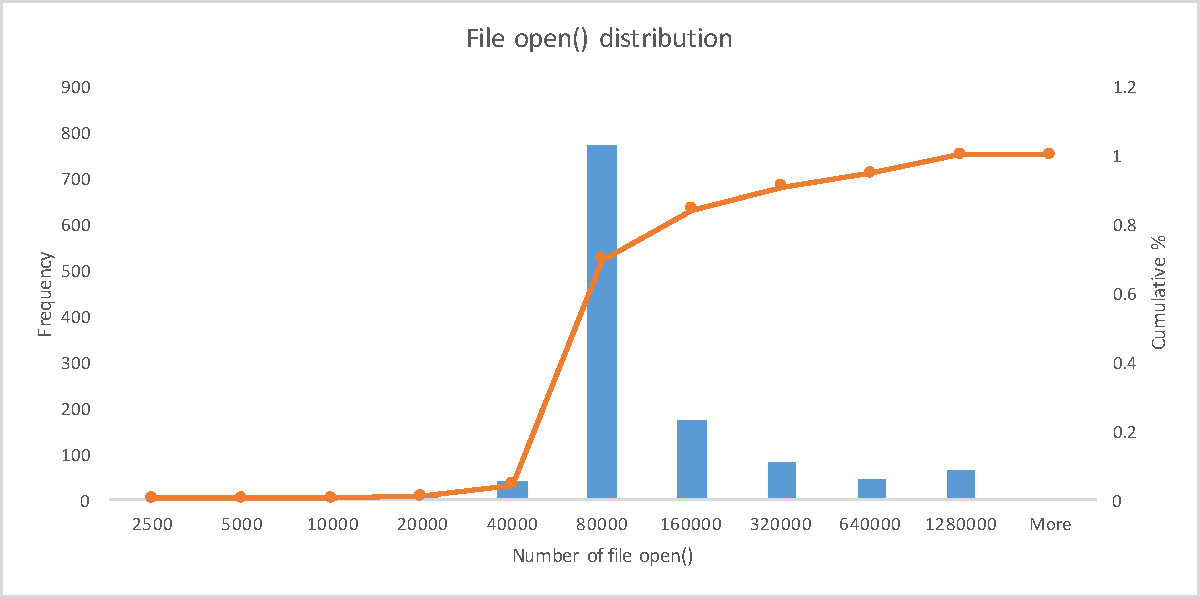
\includegraphics[width=0.48\textwidth]{figures/panda_file_open_hist.pdf}}\\
    \end{tabular}
    \caption{ATLAS file open() histogram on Titan for week of 10/25/16.}
    \label{fig:atlas-titan-file-open}
\end{figure}


\begin{figure}[!htb]
    \centering
    \begin{tabular}{cc}
        {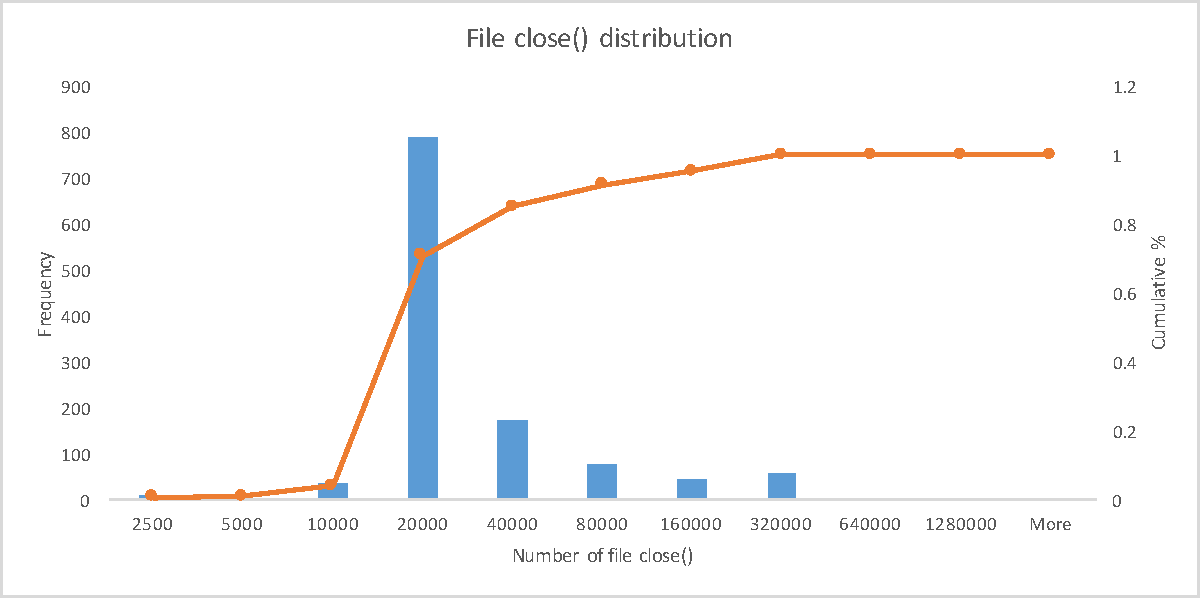
\includegraphics[width=0.48\textwidth]{figures/panda_file_close_hist.pdf}}\\
    \end{tabular}
    \caption{ATLAS file close() histogram on Titan for week of 10/25/16.}
    \label{fig:atlas-titan_file_close}
\end{figure}




\begin{table*}[t]
\centering
\begin{tabular}{lllllllll}
 & Num. Nodes & Duration (s) & Read (GB) & Written (GB) & GB Read/nodes & GB Written/nodes & open() & close() \\
Min & 1 & 1,932 & 0.01 & 0.03 & 0.00037 & 0.02485 & 1,368 & 349 \\
Max & 300 & 7,452 & 241.06 & 71.71 & 0.81670 & 0.23903 & 1,260,185 & 294,908 \\
Average & 35.66 & 6,280.82 & 20.36 & 6.87 & 0.38354 & 0.16794 & 146,459.37 & 34,155.74 \\
Std. Dev. & 55.33 & 520.99 & 43.90 & 12.33 & 0.19379 & 0.03376 & 231,346.55 & 53,799.08
\end{tabular}
\caption{The Statistical breakdown of the I/O impact of 1,175 PanDA jobs executed at OLCF for the week of 10/25/16}
\label{panda-olcf-stats}
\end{table*}
